\chapter{Scientific Background}

\section{Reference system and conventions}

In what follows, we will make use of a right-handed coordinate system, where the positive \textit{x}-axis points towards the \textit{front}, the positive \textit{y}-axis points towards the \textit{left}, and the positive \textit{z}-axis points towards the \textit{zenith} (North Pole).

Any position in the unit sphere may be described in spherical coordinates by two angles: the \textit{inclination} angle $\vartheta$, which accounts for the aperture with respect to the \textit{z}-axis, and the \textit{azimuth} angle $\varphi$, which represents the counter-clockwise angle with respect to the \textit{x}-axis from the top-view. 
The value ranges are $0 \leq \vartheta \leq \pi$ for the inclination, and $0 \leq \varphi \leq 2\pi$ for the azimuth. 

Table~\ref{tab:cartesian} shows the spherical coordinate values for some reference points on the unit sphere.
Notice that the poles ($\vartheta = �\pi$) are a special case for the spherical coordinate system -- in that case, the azimuth angle is not defined. \\


\begin{table}[!htbp]
\centering
\caption{Cartesian and spherical representation of characteristic points along the unit sphere.}
  \begin{tabular}{cccc}
  \toprule
    Position & Cartesian & $\vartheta$ & $\varphi$ \\
\midrule
	front & $[1, 0, 0]$ & $\pi/2$ & $0$ \\
	back & $[-1, 0, 0]$ & $\pi/2$ & $\pi$ \\
	left & $[0, 1, 0]$ & $\pi/2$ & $\pi/2$ \\
	right & $[0, -1, 0]$ & $\pi/2$ & $-\pi/2$ \\
    \textit{zenith} & $[0, 0, 1]$ & $0$ & * \\
    \textit{nadir}  & $[0, 0, -1]$ & $\pi$ & * \\
    \bottomrule
  \end{tabular}
\label{tab:cartesian}
\end{table}


The transformation between spherical and cartesian coordinate systems is given by the following relationship:
\begin{equation}
	\begin{aligned}
		x = & cos \varphi sin \vartheta\\
		y = & sin \varphi sin \vartheta\\
		z = & cos \vartheta\\
	\end{aligned}
\end{equation}

The \textit{elevation} angle $\theta$ provides an alternative way of describing the relationship with respect to the \textit{z}-axis. $\theta$ is defined as  the aperture with respect to the \textit{xy}-plane, with positive values towards the positive \textit{z}-axis. The relationship between elevation and inclination angles is:
\begin{equation}
	\theta = \pi/2 - \vartheta
\end{equation}


For the sake of compactness, a point in the unit sphere will be often represented by $\Omega = (\vartheta, \varphi)$.



\section{Spherical Harmonics}

\subsection{Definition}

Spherical harmonics are continuous functions defined on the sphere surface. Due to their mathematical properties, any spherical function can be decomposed as a combination of spherical harmonics, in what is known as the \textit{Spherical Harmonics Expansion} [Jarrett book, page 17].




%The spherical harmonic of \textit{order} $\ell>0$ and \textit{degree} $m$, with $|m| <= \ell$  in the direction \Omega is defined as:
Many different spherical harmonic definitions exist in the literature, with minor variations among them. In the following, we will use the real-valued, fully normalized spherical harmonics as defined by [Zotter]: 

\begin{equation}
%ambisonics book 186
	Y_n^m(\varphi, \vartheta) = N_n^{|m|} P_n^{|m|}\cos(\vartheta) \Phi_m(\varphi), 
	\label{eq:sphericalharmonics}
\end{equation}

where the \textit{normalization factor} $N_n^m$ is:

\begin{equation}
%ambisonics book 186
	N_n^m = (-1)^m \sqrt{\frac{2n+1}{2} \frac{(n-m)!}{(n+m)!}}
\end{equation}

the \textit{Legendre polynomials} $P_n^{m}$ are defined as: 

\begin{equation}
%ambisonics book 185
	P_{n+1}^{m} =
	\begin{cases}
 		\frac{2n+1}{n-m+1} x P_n^{m},  &\text{for } n = m,  \\
 		\frac{2n+1}{n-m+1} x P_n^{m} - \frac{n+m}{n-m+1}P_{n-1}^{m} &\text{else}, \\
 	\end{cases}
\end{equation}

with $P_{n}^{n} = \frac{(-1)^n(2n)!}{2^nn!}\sqrt{1-x^{2^n}}$
and the initial term $P_{0}^{0} = 1$, 

and $\Phi_m$ is the azimuthal part of the spherical harmonics: 

\begin{equation}
%ambisonics book 176
	\Phi_m(\varphi) = \frac{1}{\sqrt{2\pi}}
	\begin{cases}
    	\sqrt{2} \sin(|m|\varphi),  &\text{for } m < 0,  \\
    	1,  & \text{for } m = 0,  \\
    	\sqrt{2} \cos(m\varphi),  & \text{for } m > 0.  \\
  	\end{cases}
\end{equation}


One of the properties of the spherical harmonics is orthonormality on the sphere surface:

\begin{equation}
	\int_{\mathbb{S}^2} Y_n^m(\varphi, \vartheta) Y_{n'}^{m'}(\varphi, \vartheta) \dif cos{\vartheta} \dif \varphi = \delta_{nn'} \delta_{mm'},
	\label{eq:orthonormality}
\end{equation}

where $\delta_{xy}$ represents the Kronecker delta operator:
\begin{equation}
	\delta_{xy} = \begin{cases}
		1,  &\text{if } x = y,\\
		0,  &\text{else}.
	\end{cases}
\end{equation}

The spherical harmonics depend on the \textit{order} $n \geq 0$ and the \textit{degree} $m$,  $|m| \leq n$ for each value of $n$. In practice, the maximum order $N$, $n \leq N$ determines the spatial resolution of the sound field expansion.\\

Through the spherical harmonic expansion, any sound field may be represented with a limited spatial resolution by the finite combination of all spherical harmonics up to order $N$. 
For a given order $n$, the number of spherical harmonic functions is $2n+1$. With the accumulation of all orders up to $N$, the total number of spherical harmonics is given by $M = (N+1)^2$.
Figure~\ref{fig:sphericalharmonics} depicts all spherical harmonics from orders 0 to 3.

\begin{figure}[hbt]
  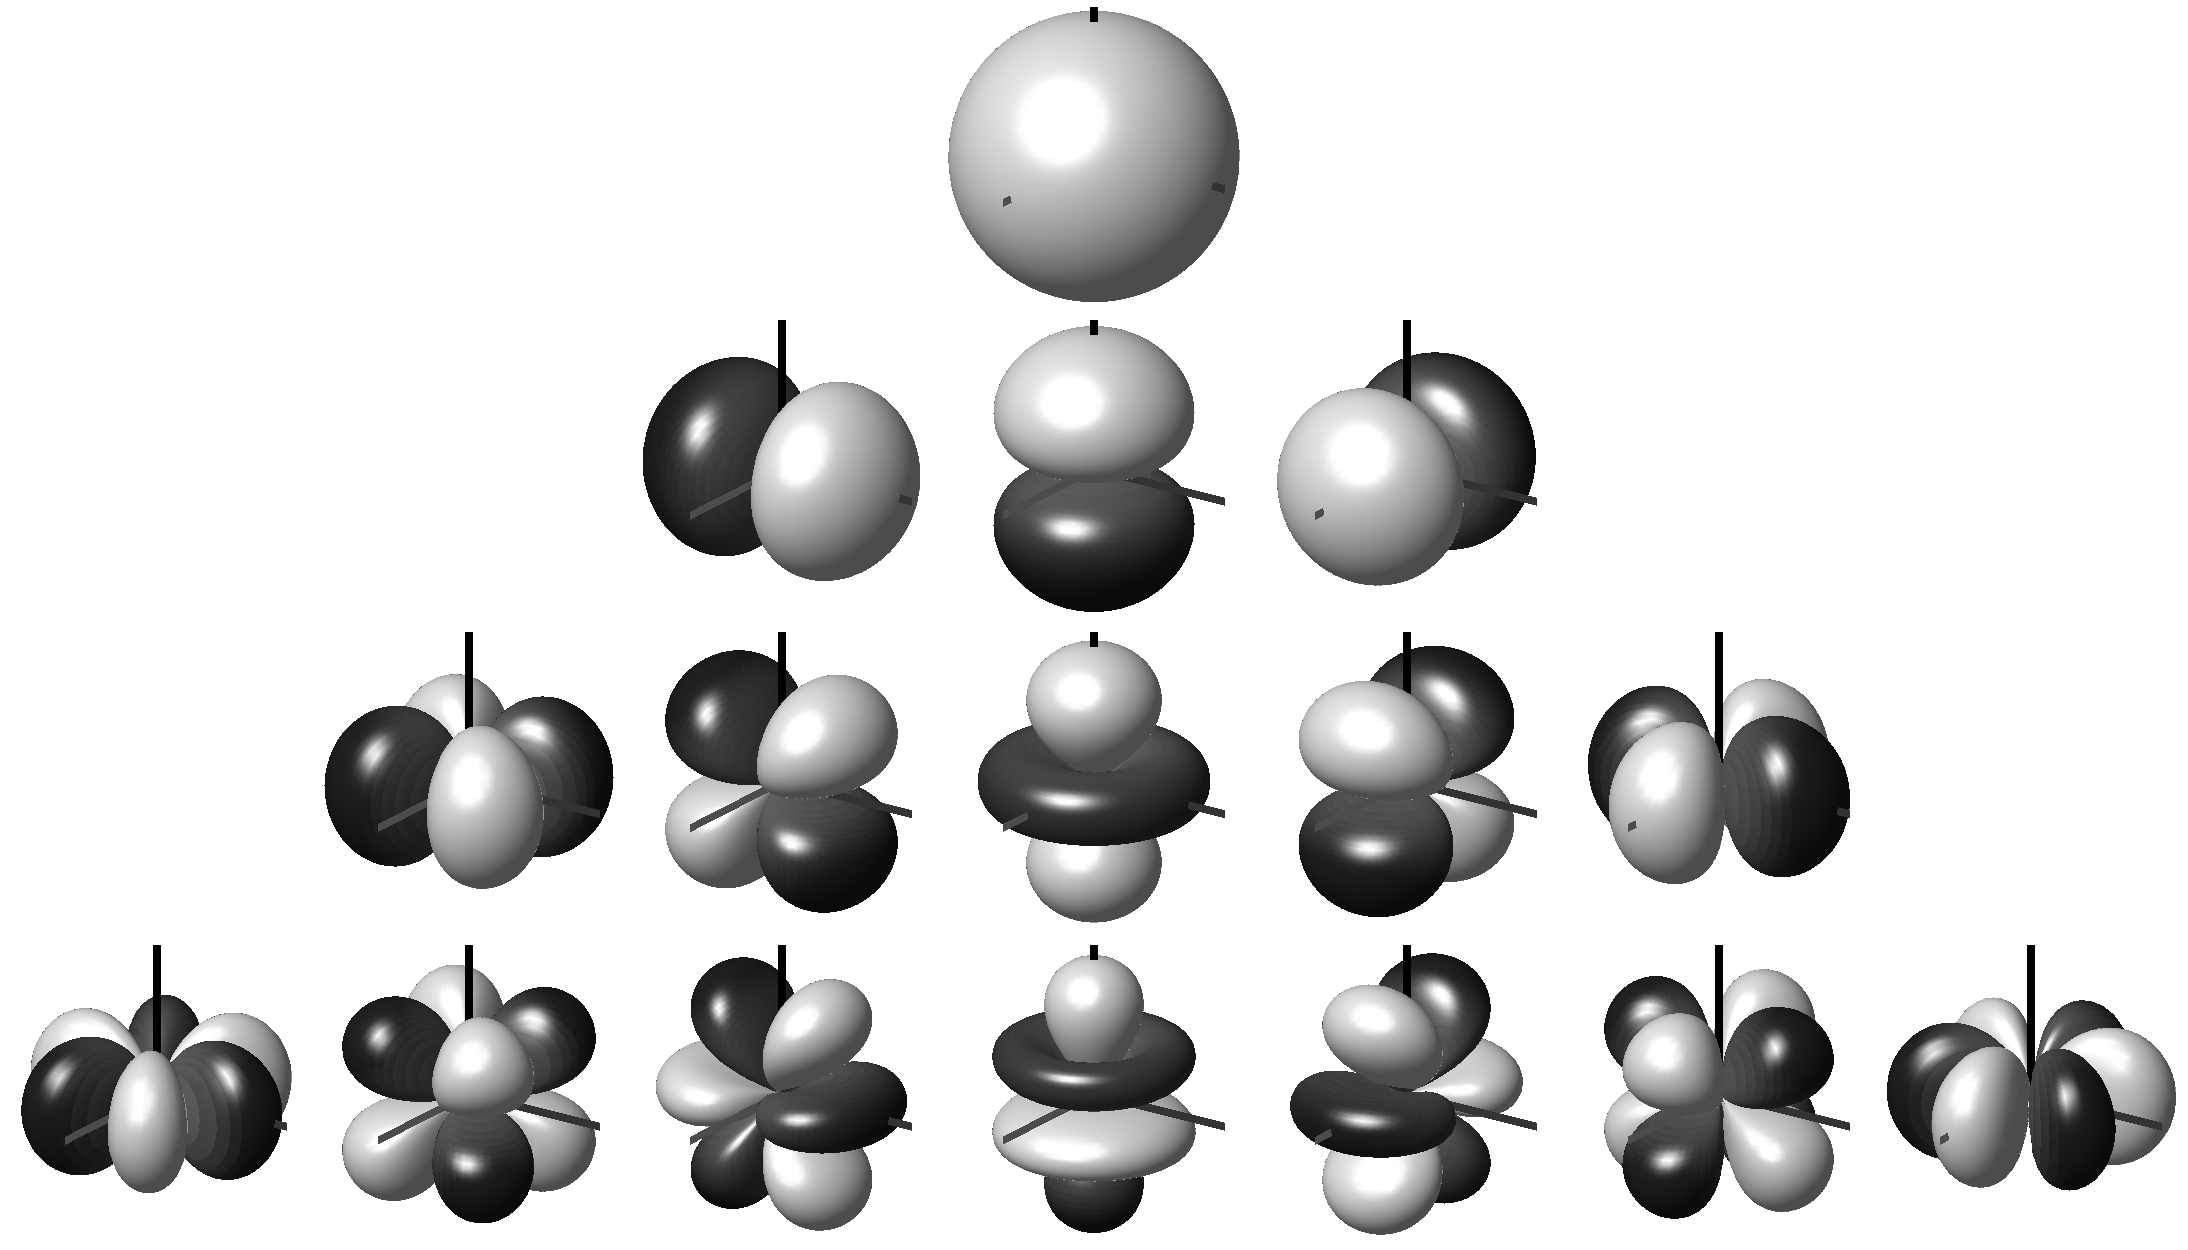
\includegraphics[width=\textwidth]{Figures/ScientificBackground/Spherical_Harmonics_deg3.png}
  \caption{Spherical harmonics up to order $N=3$. The rows correspond to the spherical harmonics of a given order $n$, and the columns span all possible degree values.}
  \label{fig:sphericalharmonics}
\end{figure}


\subsection{Spherical array processing}

Let us consider a sound field captured with a spherical microphone array, which contains $Q$ capsules distributed around a spherical surface of radius $R$ at the positions $\Omega_q, 1 \leq q \leq Q$. 
The captured frequency-domain signals $X_q(k)$ can be represented as the spherical harmonic domain signals $X_n^m(k)$ through the spherical harmonic transform of order $n$ and degree $m$ (Moreau et al., 2006):

\begin{equation}
	X_n^m(k) = \sum_{q=1}^{Q} X_q(k) Y_n^m(\Omega_q) \Gamma_n(kR),
	\label{eq:a2b}
\end{equation}
\todo{is that actually valid? or Y should be the complex-valued spherical harmonics?}

where the term $\Gamma_n(kR)$ models the radial transfer function, and depends on the microphone geometry[SOME REFS: moreau, rafaely]. There are several possible sampling schemes of capsules along the sphere, each one having different properties; the reader is redirected to [rafaely] for a deeper insight. \\

By using this model, the maximum spherical harmonic order $N$ that can be retrieved with negligible spatial aliasing depends on the number of microphone capsules [moreau]:
\begin{equation}
	N \geq (Q + 1)^2.
\end{equation}

Furthermore, the sphere radius $R$ has also an effect on the operational bandwidth of the microphone. More precisely, for a given spherical harmonic order $n$, the maximum aliasing-free operational frequency is given by [moreau, rafaely]:
\begin{equation}
	f_{max} = \frac{n c} {2 \pi R},
	\label{eq:falias}
\end{equation}

with $c$ being the sound speed.

\todo{moreau has c/2Rgamma}.




\section{Ambisonics}

\subsection{Ambisonics Theory}

Ambisonics is a spatial sound recording and playback technology initially developed during the 1970's, and further expanded into its modern formulation around the 2000s [ZOTTER, page 53].  
Ambisonics is based on the idea of decomposing a sound field into its spherical harmonic representation. 

Originally, the decomposition was limited to first-order spherical harmonics, mainly due to practical limitations [CITE GERZON], as the so-called \textit{First Order Ambisonics} (FOA). The technique was later formalized for arbitrary spherical harmonic orders, known as \textit{Higher Order Ambisonics} or HOA [CITE DANIEL].
In general, with the term Ambisonics we will be referring to the latter definition.\\

\subsubsection{Ambisonic encoding}

Let us consider a sound field composed of a point sound source $S$ located in far-field at the angular position $\Omega_s$. The sound pressure at the coordinate origin can be expressed in terms of the spherical harmonic expansion of order $N$ as: \todo{check equation, find references, how to explain the domain? extend also to multiple sources by superposition}
\begin{equation}
	P = \sum_{n=0}^{N} \sum_{m=-n}^{n} Y_n^m(\Omega_s) S
	\label{eq:encoding}
\end{equation}


The ordered set of values of all spherical harmonics up to order $N$, evaluated at the source position, is known as the \textit{ambisonic coefficients}:
\begin{equation}
	\pmb{Y}_n^m(\Omega_s) = [Y_0^0(\Omega_s), Y_1^{-1}(\Omega_s),  \ldots ,  Y_N^N(\Omega_s)]
	\label{eq:sphericalharmonicvector}
\end{equation}

Furthermore, the process of multiplying the signal $S$ by the ambisonic coefficients is known in the literature as the \textit{ambisonic encoding}. The resulting signal vector is usually referred to as the \textit{ambisonic} (or \textit{B-Format}) signal $\pmb{S}_n^m$:
\begin{equation}
	\pmb{S}_n^m = \pmb{Y}_n^m(\Omega_s) S
\end{equation}


Although the term \textit{B-Format} was initially introduced as an alternative name for first-order ambisonic signals [gerzon, tesis de daniel], it is nowadays common to use it as a synonim of ambisonic signals, without any order restriction. We will use the latter acception in what follows.

Historically, the name \textit{B-Format} was used as an opposite of \textit{A-Format}, which describes the signals recorded by a tetrahedral microphone array [cite gerzon?]. The tetrahedron is the simplest and most common form of spherical microphone arrays (\textit{ambisonic microphones}) with uniform capsule distribution. Again, the term \textit{A-Format} is also currently employed for referring to the signals recorded by any spherical microphone array, regardless of the number or arrangement of capsules.

Likewise, the process of signal conversion from the spatial domain (microphone capsules) to the spherical harmonic domain (ambisonic signals), as in Eq.~\ref{eq:a2b}, is known as \textit{A-B conversion}. A number of different approaches have been developed for this process, and the interested reader is referred to [\todo{find ref}] for more information.

In practice, there are two alternative ways to generate ambisonic signals. The first one is the \textit{synthesis}, based on the direct application of ambisonics encoding (Eq.~\ref{eq:encoding}) to a monophonic signal. The second one is the \textit{recording} with a spherical microphone array, followed by the aforementioned domain conversion. \\


\subsubsection{Ambisonic Decoding}
Conversely, the sound field reconstruction is performed by the \textit{ambisonic decoding} operation. This process is equivalent to weight-and-sum beamforming in the spherical harmonic domain, and it is sometimes also referred to as the \textit{virtual microphone} technique [ambisonic book].

\todo{change L for other name}
Let us consider a loudspeaker located at the angular position $\Omega_\ell$. The signal feed $L$ is \textit{decoded} from the ambisonic signal as:
\begin{equation}
	L = \sum_{n=0}^{N} \sum_{m=-n}^{n} Y_n^m(\Omega_s) Y_n^m(\Omega_\ell)  S \alpha_n 
	\label{eq:decoding}
\end{equation}

where $\alpha_n$ is a weighting factor which accounts for the beam directivity. Some of the weightings are widely used for its specific properties, such as \textit{max-rE} or \textit{in-phase} -- the reader is referred to [\todo{find ref. daniel? zotter?}] for more information.

The decoding equation \ref{eq:decoding} can be written in vector form as:
\begin{equation}
	L =  \pmb{S}_n^m {\pmb{Y}_n^{m}(\Omega_\ell)}^T \alpha_n
\end{equation}

where the superscript $T$ represents the matrix transposition. 
This equation can be extended to the regular case of decoding to a loudspeaker array, comprised of $L$ loudspeakers located at the positions $\pmb{\Omega}_l = [\Omega_{\ell_1}, \ldots, \Omega_{\ell_L}]$ . In such case, the loudspeaker feed vector $\pmb{L}$ can be written as:
\begin{equation}
	\pmb{L} = \pmb{S}_n^m \pmb{D},
\end{equation}
where 
\begin{equation}
	\pmb{D} = \text{diag}(\alpha_n) [{\pmb{Y}_n^{m}(\Omega_{\ell_1})}^T, \ldots, {\pmb{Y}_n^{m}(\Omega_{\ell_L})}^T]
\end{equation}

is a $M \times L$ matrix known as the \textit{decoding matrix}, and $\text{diag}(\alpha_n)$ is a diagonal matrix of size $M$ containing the values of $\alpha_n$ along the main diagonal. 
$\pmb{D}$ is frequency-independent and depends solely on the loudspeaker array geometry. The reader is referred to [zotter? daniel? idhoa?] for more information about the vast field of study of ambisonic decoding.

\todo{figure from daniel? to sum up the subsection). Explain the allrad method and stuff because it will appear later on}.



\subsection{Practical considerations}

Due to historical and practical reasons, there are two aspects that must be taking into account when working with ambisonic signals: \textit{channel normalization} and \textit{channel ordering}. 
In the following, the term \textit{channels} will be used as a synonym for spherical harmonics, as they are usually referred to in sound engineering contexts\footnote{In fact, ambisonic signals are inherently multichannel, even though each channel corresponds to a spherical harmonic, and not to a loudspeaker feed as in traditional \textit{channel-based} audio.}.  \\


\subsubsection{Channel normalization}
Let us consider the spherical harmonics $Y_n^m(\Omega)$ as defined in Eq.~\ref{eq:sphericalharmonics}. Due to the orthonormal property showed in Eq.~\ref{eq:orthonormality}, they follow the \textit{fully 3d normalized} or \textit{N3D} channel normalization convention. \todo{what about the 1/sqrt(4pi)???}. 

Alternatively, the \textit{Schmidt 3d semi-normalized} or \textit{SN3D} [daniel] convention is also of widespread usage. The conversion between \textit{N3D} and \textit{SN3D} is driven by the following expression:
\begin{equation}
	{Y_n^m(\Omega)}^{\text{(N3D)}} = \sqrt{2n+1} {Y_n^m(\Omega)}^{\text{(SN3D)}}
\end{equation}

\textit{MaxN} is another existing convention. It defines all spherical harmonics as having a maximum absolute value of 1: 
\begin{equation}
	\max_{\Omega} |{Y_n^m(\Omega)}^{\text{(MaxN)}}| = 1, \forall (n, m)
\end{equation} 

Finally, the \textit{Furse-Malham} (or \textit{FuMa}) normalization only differs from \textit{Max-N} in the scaling of the zero-th order component: 
\begin{equation}
	{Y_n^m(\Omega)}^{\text{(FuMa)}} = \begin{cases}
		1 / \sqrt{2},  &\text{if } n = 0,\\
		{Y_n^m(\Omega)}^{\text{(MaxN)}},  &\text{else}.
	\end{cases}	
\end{equation} 

Each of the normalization schemes has its own particularities. For instance, \textit{N3D} is the most mathematically straightforward, and spherical harmonics defined in that way can be directly used for both encoding and decoding (as in Eqs~\ref{eq:encoding} and Eq.~\ref{eq:decoding}) -- however, from a sound engineer point of view, other normalization schemes with maximum values below the unity might be preferred, such as \textit{SN3D}. Besides this, \textit{FuMa} has been historically the default normalization \todo{[gerzon?]}, while the more modern \textit{N3D} and \textit{SN3D} were popularized after Daniel \todo{[daniel]}. \\

\begin{figure}[hbt!]
  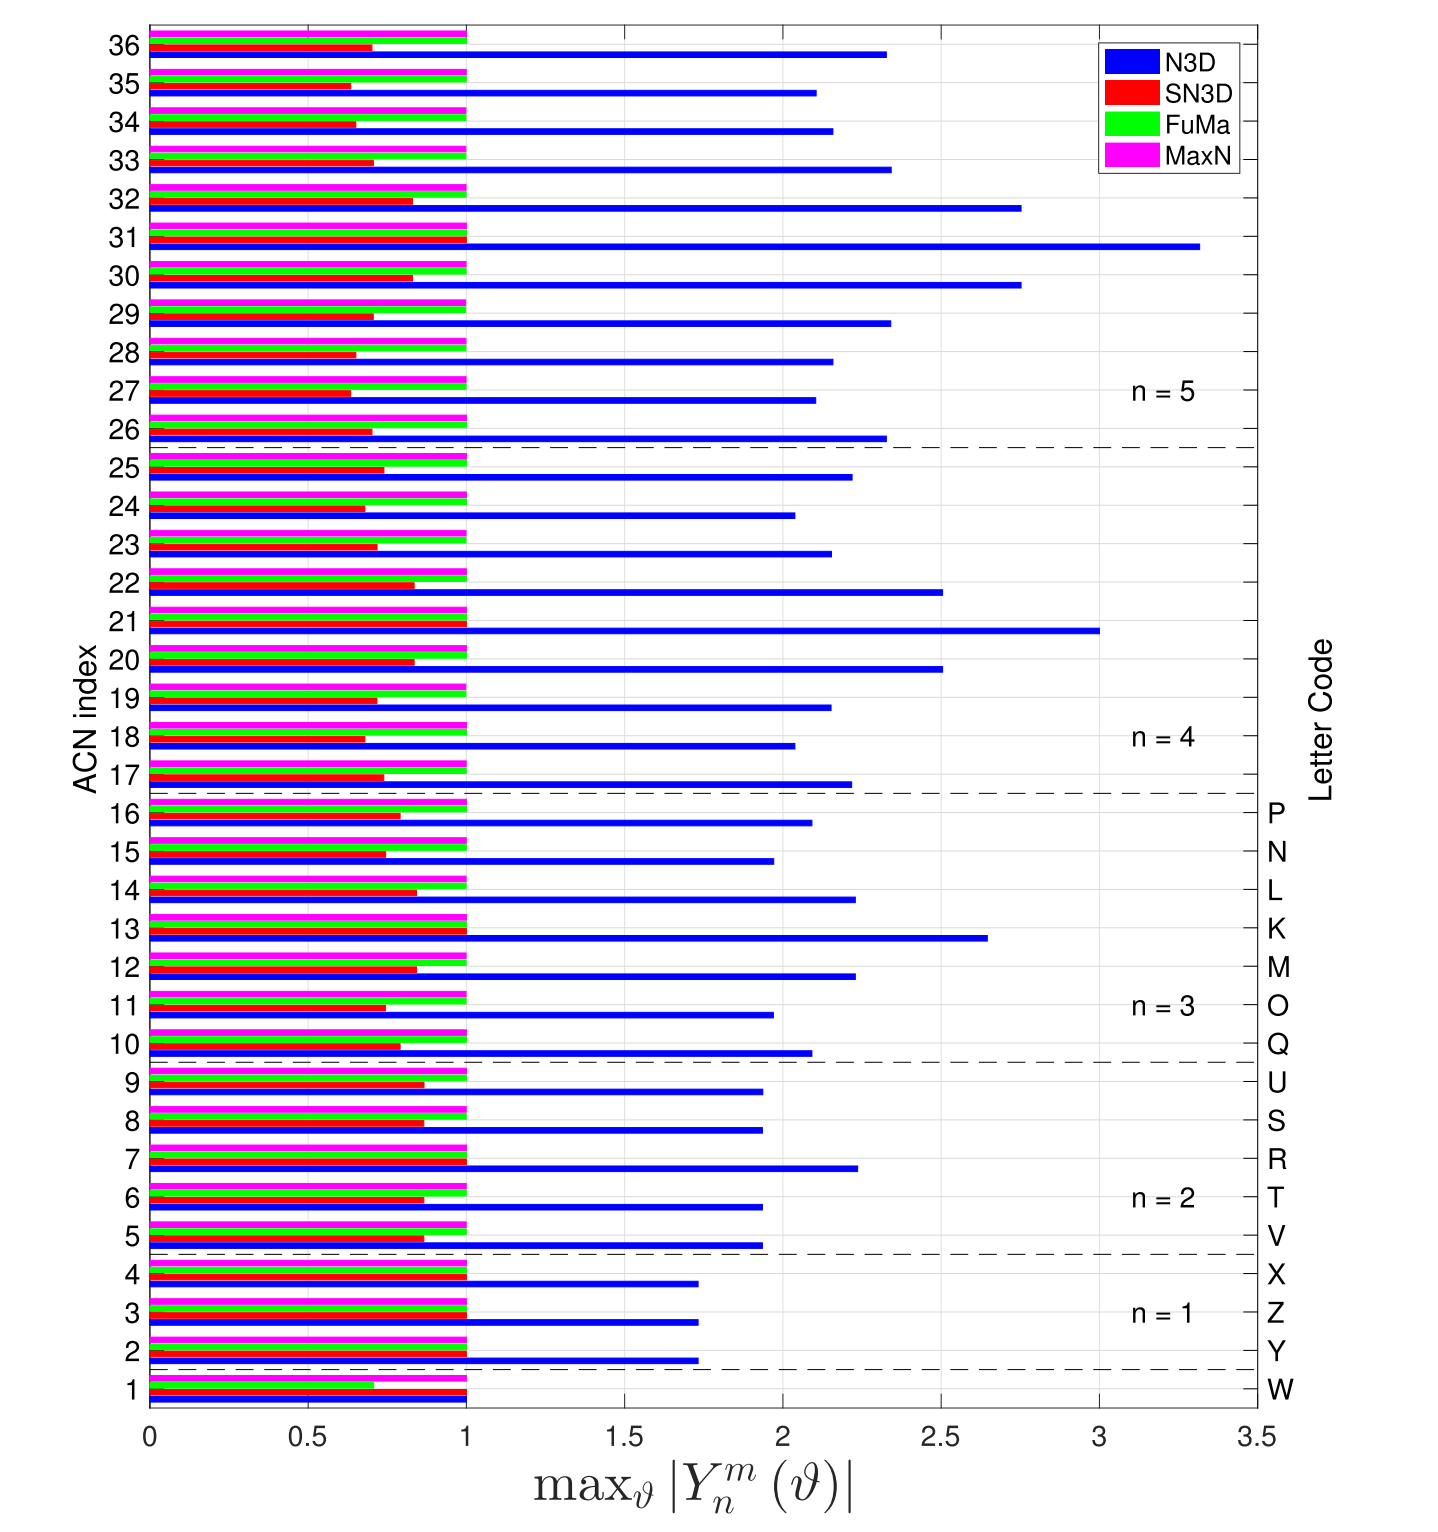
\includegraphics[width=\textwidth]{Figures/ScientificBackground/normalization.png}
  \caption{Maximum value of each ambisonic channel up to order 5, for all different normalization schemes. Image from T. Carpentier [\todo{cite}].}
  \label{fig:normalization}
\end{figure}


As a summary, Figure~\ref{fig:normalization} displaysthe different normalization schemes. The reader is referred to \todo{[thibaut]} for an extensive review on the topic.



\subsubsection{Channel ordering}

Channel ordering refers to the manner in which spherical harmonics, inherently organized in the 2D space by dimensions $n$ and $m$, are sorted into a one-dimensional vector. 

The \textit{ACN} (from \textit{Ambisonic Channel Number}) scheme follows from the mathematical description given in Eq.~\ref{eq:sphericalharmonicvector}. The spherical harmonics are first ordered by ascending order $n$ and, inside each order, by ascending degree $m$. The index of a given channel $i \in [0 \ldots M-1]$ can be thus obtained by the following relationship:
\begin{equation}
	i = n^2 + n + m 
\end{equation}

Historically, first-order ambisonic audio has followed what it might be called \textit{traditional B-Format} channel ordering [ambisonics in multichannel broadcasting and video]. 
By following this scheme, the four channels are referred to by the axis where the corresponding spherical harmonic steers, plus the name $W$ for the zeroth order component:
\begin{equation}
	{\pmb{Y}_n^m(\Omega)}^{\text{(FuMa CO)}} = [W, X, Y, Z]
\end{equation}
with:
\begin{equation}
\begin{aligned}
	&W = Y_0^0(\Omega) \\
	&X = Y_1^1(\Omega) \\
	&Y = Y_1^{-1}(\Omega) \\
	&Z = Y_1^0(\Omega)
\end{aligned}	
\end{equation}

This nomenclature was extended to second and third order by Malham, and is currently known as the \textit{Furse-Malham} or \textit{FuMa} channel ordering. The channel names use all english alphabet letters from K to Z in third order and, although there would be enough letters to go up to fourth order, the unconvenience of the system was evident [Higher order Ambisonic systems].
Figure~\ref{fig:normalization} shows the equivalence between \textit{FuMa} (\textit{"letter code"}) and \textit{ACN} channel names.\\


In practice, there exist two main combinations of channel normalization and ordering schemes:
\begin{itemize}
  \item The \textit{classical} approach, usually limited to first-order ambisonics, which uses \textit{FuMa} normalization and channel ordering\footnote{In general, it may be expected that \textit{early} ambisonic material follow these conventions without any explicit mention to them.}.
  \item The \textit{modern} approach, inspired by the \textit{ambix} file format [cite ambix], with \textit{SN3D} normalization and \textit{ACN} channel ordering.
\end{itemize}

Anyhow, the \textit{classical B-Format} channel naming and ordering is still widely used when referring to first-order ambisonics. In what follows, we will use indistinctly both \textit{classical} and \textit{ACN} conventions. \todo{is that true?}


\section{Parametric Spatial Audio Analysis}

Trough parametric analysis, sound fields may be described in terms of a small amount of sound sources and associate parameters. Such representation might reduce to a great extent the complexity of processing methods [book jarrett].

One of the most successful sound field parametric models is DirAC[pulkki2007 dirac]. Originally conceived as a method for impulse response processing and spatial sound reproduction [merima2005], it has been widely used in many different audio-related problems [\todo{find some references!}].

DirAC (acronym for \textit{Directional Audio Coding}) is a perceptually motivated time-frequency domain method, based on the assumption that any sound field may be reproduced with high perceptual quality by considering two parameters: the sound field diffuseness and the most prominent sound direction of arrivals (DOAs) [cite parametric book]. \\

Let us consider a \textit{N3D}-normalized first-order ambisonic signal in time-frequency domain $\pmb{B}_n^m(k, n)$, begin $k$ the frequency index and $n$ the time index. For the sake of clarity, we will use \textit{FuMa} channel notation and ordering:
\begin{equation}
	\pmb{B}_n^m(k, n) = [W(k, n), X(k, n), Y(k, n), Z(k, n)]
\end{equation}

Given this representation, we can express the \textit{pressure} $P(k,n)$ of the sound field as:
\begin{equation}
	P(k,n) = W(k,n)
\end{equation}
as well as the sound \textit{pressure-gradient} (or \textit{velocity}) $\pmb{U}(k,n)$ as: 
\begin{equation}
	\pmb{U}(k,n) = - \frac{1}{\rho_0 c} [X(k, n), Y(k, n), Z(k, n)], 
\end{equation}
where $\rho_0$ is the mean density of the medium, and $c$ is the speed of sound.\\ 

The \textit{active intensity} $\pmb{I}(k,n)$, defined as the amount of transmitted acoustic energy, can be expressed in terms of sound pressure and velocity [fahy2002]:
\begin{equation}
	\begin{aligned}
	\pmb{I}(k,n) &=  \Re\{P^*(k,n)\pmb{U}(k,n)\} \\
	&= - \frac{1}{\rho_0 c}\Re\{W^*(k,n)[X(k,n),Y(k,n),Z(k,n)]\},
	\end{aligned}
\end{equation}
where $^*$ represents the complex conjugate operator. \\

An estimate of the instantaneous DOA $\Omega(k,n)$ can be extracted from the intensity vector, interpreting each of its time-frequency bins as a point in the cartesian space. Effectively, the sound propagation direction is the opposite to the observed arrival direction. 
\begin{equation}
	\Omega(k,n) = \angle(-\pmb{I}(k,n)),
\end{equation}
with $\angle$ representing the spherical angle operator of a cartesian vector. The result of this computation must be understood as the direction of the net energy flow, which in the case of a single plane-wave will correspond to the source position. \\

Another useful parameter is the \textit{energy density} $E(k,n)$ [stazial 1996]:
\begin{equation}
	\begin{aligned}
		E(k,n) &= \frac{|P(k,n)|^2 + \|\pmb{U}(k,n)\|^2}{2\rho_0 c^2} \\ 
		&=  \frac{|W(k,n)|^2 + \| [X(k,n), Y(k,n), Z(k,n)] \|^2}{2\rho_0 c^2}.
	\end{aligned}
\end{equation}\\

Finally, the \textit{diffuseness} $\Psi(k,n)$ can be computed from the sound intensity and  energy density [merimaa2005]:
\begin{equation}
	\begin{aligned}
		\Psi(k,n) &= 1 - \frac{ \| \langle \pmb{I}(k,n) \rangle \| }{ c \langle E(k,n) \rangle } \\
		&= 1 - 2\frac{ \| \langle \Re\{W^*(k,n)[X(k,n),Y(k,n),Z(k,n)]\} \rangle \| }{ \langle |W(k,n)|^2 + \| [X(k,n), Y(k,n), Z(k,n)] \|^2 \rangle },
	\end{aligned}
	\label{eq:psidefinition}
\end{equation}
 
 where the symbols $\langle \cdot \rangle$ represent the expectation operator, which is usually implemented as time-domain averaging. \todo{check equation}

Even though Eq.~\ref{eq:psidefinition} (known as \textit{DirAC's diffuseness}) is one of the most common ambisonic diffuseness estimators, several alternative formulations exist. 
Other diffuseness estimation procedures include the \textit{coefficient of variation method} [ahonen, pulkki, del galdo] and the more recent \textit{COMEDIE} estimator [epain, craig]. 

In any case, in what follows, the term \textit{diffuseness} and the symbol $\Psi$ will refer by default to Eq.~\ref{eq:psidefinition}.  \\


As a mathematical convenience, we will define the \textit{B-Format coherence} as the complement of the diffuseness:
\begin{equation}
	\Delta(k,n) = 1 - \Psi(k,n) 
	\label{eq:delta}
\end{equation}


\section{Spatial Coherence Analysis}
\todo{put this chapter in context or something}\\


In the context of microphone array signal processing, diffuseness is commonly estimated through the
\textit{Magnitude Squared Coherence} (MSC) \cite{elko_spatial_2001} between two frequency-domain signals $S_1$ and $S_2$, as a function of the
\textit{wavenumber} $k$ and the microphone distance $r$:
\begin{equation}
    \text{MSC}_{12}(k r) =
	\frac{|\left\langle S_1(k r) S_2(k r)^* \right\rangle|^2}
	{\left\langle|S_1(k r)|^2\right\rangle \left\langle|S_2(k r)|^2\right\rangle},
    \label{eq:MSC}
\end{equation}
where the $\left\langle \cdot \right\rangle$ operator represents the temporal
expected value, and $^*$ defines the complex conjugate operator. In the case of spherical isotropic noise fields, Eq.~(\ref{eq:MSC})
can be expressed in terms of microphone directivity patterns
$T(\phi,\theta,k r)$ as \cite{elko_spatial_2001}:

\begin{equation}
	\begin{aligned}
&\text{MSC}_{12}(k r) = \frac{|N_{12}(k r)|^2}{|D_{12}(kr)|^2} \\
&= \frac{|\int_{0}^{\pi} \int_{0}^{2\pi} T_1(\phi,\theta,k r) T_2^*(\phi,\theta,k r) e^{-jk r cos\theta} sin\theta d\theta d\phi|^2}{|\sqrt{ \int_{0}^{\pi} \int_{0}^{2\pi} |T_1(\phi,\theta,k r)|^2 sin\theta d\theta d\phi } \sqrt{\int_{0}^{\pi} \int_{0}^{2\pi}|T_2(\phi,\theta,k r)|^2 sin\theta d\theta d\phi}|^2}.
\label{eq:MSCdir}
    \end{aligned}
\end{equation}


Moreover, the general expression of the directivity of a first-order differential microphone is given by the following relationship:

\begin{equation}
	\begin{aligned}
	T_i(\Omega_i) = \alpha_i + (1 - \alpha_i) \cos{\Omega_i},
	\end{aligned}
\end{equation}


where $i \in [1,2]$ is the microphone index, $\Omega_i$ is the angle between wave incidence and microphone orientation axis, and $\alpha_i \in [0,1]$ is the directivity parameter of the microphone $i$, which ranges from bidirectional ($\alpha_i = 0$) to omnidirectional ($\alpha_i = 1$). \\


For first-order differential microphones, there is a closed-form expression for the numerator and denominator of Eq.~(\ref{eq:MSCdir}):
\begin{equation}
	\begin{aligned}
    &N_{12}(k r) =  \frac{\alpha_1 \alpha_2 sin(kr)}{kr} \\
    &+ \frac{(1-\alpha_2)(1-\alpha_2)(x_1x_2+y_1y_2)}{(kr)^3}(sin(kr)-kr cos(kr)) \\
    &+ \frac{z_1 z_2}{kr^3}[ ( (kr)^2 sin(kr) + 2kr cos(kr) )(1-\alpha_1)(1-\alpha_2) 
    + 2 sin(kr)(1-\alpha_1)(1-\alpha_2) ] \\
    &+ \frac{z_1}{(kr)^3}[ j(kr)^2 \alpha_2 cos(kr)(\alpha_1-1) + jkr \alpha_2 sin(kr)(1+\alpha_1) ] \\
    &+ \frac{z_2}{(kr)^3}[ j(kr)^2 \alpha_1 cos(kr)(\alpha_2-1) + jkr \alpha_1 sin(kr)(1+\alpha_2) ],\\
    &D_{12}(kr) =  \frac{\sqrt{3 \alpha_1^2+(1-\alpha_1)^2}\sqrt{3 \alpha_2^2+(1-\alpha_2)^2}}{3},
    \label{eq:closedform_msc}
    \end{aligned}
\end{equation}
where $x_i$, $y_i$ and $z_i$ are the cartesian coordinates of the wave incidence angle $\Omega_i$. \todo{check}.





\section{Room Acoustics, Impulse Responses}


\section{SOFA}
 maybe as subsection of room acoustics


%
%
%
%sound field capturing
%
%spherical harmonics
%
%decoding/beamforming
%
%\subsection{normalization, channel ordering}
%
%\section{Parametric spatial analysis}
%
%sirr, dirac
%
%sound field pressure and velocity approximation
%
%intensity vector
%direction of arrival
%energy density
%diffuseness (limits)

%alternative formulations



\section{Practical Considerations}

